\section{Results}
\label{sec:results}

Every wall time below is a median of the measured repeats in \texttt{results/runs.csv}. The main curves use five repeats after one discarded warmup. Chunk size, block size, the single-month run, and the weak-scaling runs use three. Quartile bands on Figure~\ref{fig:speedup} use the first and third quartiles of wall time and the same $T_1$. The page cache was not dropped.

\subsection{Trip groups}
\label{sec:clusters}

The grouping run is separate from the timing kernel. It draws 25{,}000 cleaned rows from each of the twelve 2023 files, keeps the 299{,}970 rows with a zone centroid, and fits 200{,}000 of those rows. The six features are the zone centroid's easting and northing, $\sin(2\pi h/24)$ and $\cos(2\pi h/24)$ for the pickup hour $h$, a weekend indicator, and $\log(1 + \text{distance})$. Each column is standardised to zero mean and unit variance. Easting and northing are the TLC shapefile's State Plane coordinates (NAD83, New York Long Island, US survey feet). A Euclidean distance in degrees of longitude and latitude would stretch the east-west axis, so the projected coordinates are the ones in the file.

Labels use the row-order centroid update, for 30 iterations, so they do not depend on the thread count. Silhouette is computed earlier, on 8{,}000 of the fitted rows, after 20 iterations. Table~\ref{tab:sil} is that curve. The maximum is $k = 2$ at 0.550. The score falls to 0.266 at $k = 3$ and is 0.312 at $k = 4$ and 0.322 at $k = 5$.

\begin{table}[ht]
\centering
\caption{Silhouette on 8{,}000 of the 200{,}000 fitted rows. Euclidean distance in the six standardised features. The maximum is $k = 2$. The groups in Table~\ref{tab:clusters} use $k = 4$.}
\label{tab:sil}
\begin{tabular}{cccccccc}
\toprule
$k$ & 2 & 3 & 4 & 5 & 6 & 7 & 8 \\
\midrule
Score & 0.550 & 0.266 & 0.312 & 0.322 & 0.308 & 0.263 & 0.308 \\
\bottomrule
\end{tabular}
\end{table}

The $k = 2$ fit is a length and borough split. One group has 188{,}888 rows (94.4\%), mean distance 2.76 miles, mean hour 14.3, and 95.0\% Manhattan. The other has 11{,}112 rows (5.6\%), mean distance 16.1 miles, mean hour 14.6, and 99.7\% Queens. The two mean hours differ by 0.3 hours. A higher silhouette here is one airport against the city, not a split by time of day.

We report $k = 4$, not the silhouette maximum. The $k = 5$ score is 0.010 higher than $k = 4$, and the fifth group is a night cluster that mixes weekdays and weekends. The four groups in Table~\ref{tab:clusters} each have one reading. Cluster 3 is weekday morning and midday (mean hour 10.5, weekend share 0, midday share 64.7\%). Cluster 0 is weekday afternoon and evening (mean hour 17.7, weekend share 0, afternoon plus evening 67.8\%). Cluster 2 is the weekend (weekend share 100\%, mean hour 13.3). Cluster 1 is the JFK group (99.7\% Queens, mean distance 16.1 miles, mean duration 42.0 minutes, mean fare \$63.69). Mean distance in the three Manhattan groups stays between 2.68 and 2.84 miles.

\begin{table}[ht]
\centering
\caption{k-means profiles on 200{,}000 trips from 2023, $k = 4$. Cluster ids are the labels from the fit. The order of columns follows the reading in the text, not the id order.}
\label{tab:clusters}
\small
\setlength{\tabcolsep}{5pt}
\begin{tabular}{lrrrr}
\toprule
 & C3 & C0 & C2 & C1 \\
\midrule
Rows & 58,084 & 79,950 & 50,874 & 11,092 \\
Share & 29.0\% & 40.0\% & 25.4\% & 5.5\% \\
Mean distance (miles) & 2.81 & 2.68 & 2.84 & 16.10 \\
Mean duration (minutes) & 15.8 & 14.6 & 13.9 & 42.0 \\
Mean fare (USD) & 17.80 & 16.67 & 16.82 & 63.69 \\
Mean pickup hour & 10.5 & 17.7 & 13.3 & 14.6 \\
Weekend share & 0\% & 0\% & 100\% & 28.7\% \\
Manhattan share & 94.7\% & 94.9\% & 95.4\% & 0\% \\
Queens share & 4.9\% & 4.8\% & 4.0\% & 99.7\% \\
\bottomrule
\end{tabular}
\end{table}

Cluster 1 is one airport, not the borough. Zone 132, JFK Airport, accounts for 10,903 of its 11,092 rows, or 98.3\%. The other 189 rows are spread over 41 zones: 161 rows in 24 other Queens zones, and 28 rows in 17 Brooklyn zones. LaGuardia, zone 138, is not in this group. Its 7,243 sampled pickups fall in clusters 0, 2, and 3. The remaining Queens pickups are not lost. Clusters 0, 2, and 3 draw 4.8\%, 4.0\%, and 4.9\% of their rows from Queens, and their mean distance stays between 2.68 and 2.84 miles. Only the JFK trips are long and expensive enough to stand apart. That reading matches the fare spike in Section~\ref{sec:eda}.

Weekend share is 0 or 1 in the three Manhattan groups because the weekend indicator is one of the six inputs. That cluster is the coordinate being used, not a pattern found in spite of it. The morning and afternoon split is not a pre-cut label: the clock enters only as $\sin$ and $\cos$ of the hour. The airport group agrees in both geography and distance. Its zone centroid sits far from Manhattan, and its mean distance is 16.1 miles against 2.7--2.8 miles in the other three groups. We did not drop either feature, so this fit does not say which of the two is sufficient. The four groups are the $k = 4$ cut of this feature set. $k = 2$ remains the silhouette maximum, and it is the same airport tail before the clock is split.

\begin{figure}[ht]
\centering
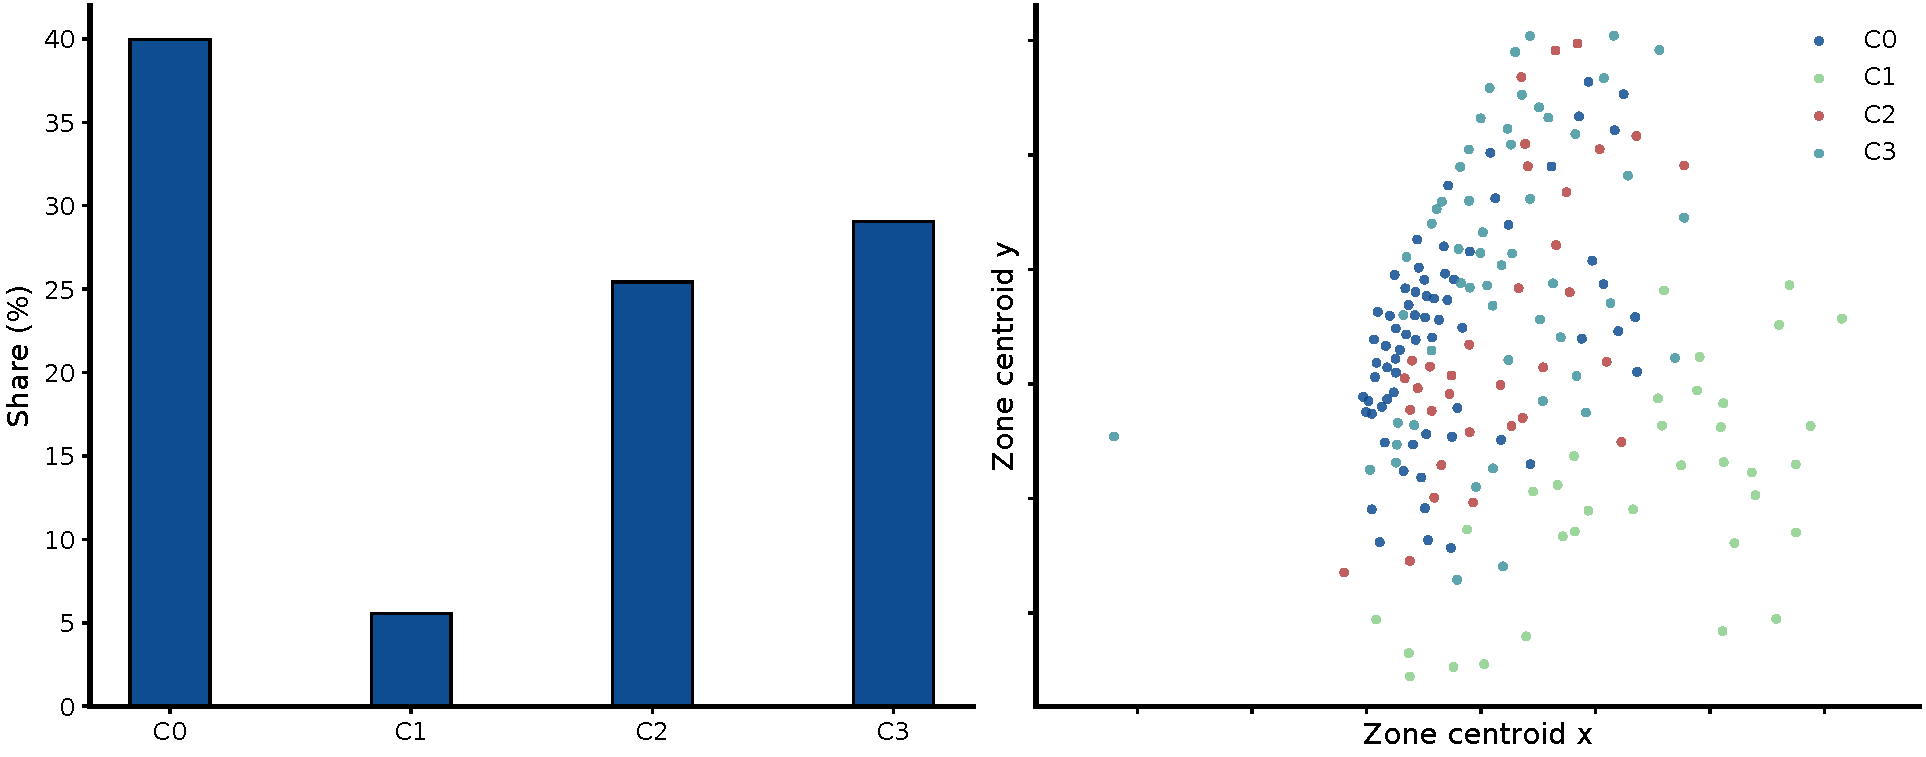
\includegraphics[width=\textwidth]{fig07_clusters}
\caption{Left: share of the 200{,}000 fitted rows. Right: zone centroids coloured by the majority cluster among sampled pickups in that zone. The three Manhattan groups share the same zones, so the majority colour on Manhattan is cluster 0, the larger weekday group. Zone 132, JFK Airport, takes cluster 1. A few neighbouring Queens zones share that colour on a small sample. Cluster 2, the weekend, has no zone of its own.}
\label{fig:clusters}
\end{figure}

\FloatBarrier
\subsection{ETL: processes, threads, and chunk size}
\label{sec:speedup}

Figure~\ref{fig:speedup} plots $S(p)$ for the ETL, the k-means kernel, and FP-Growth. The dashed line is $S(p) = p$. Table~\ref{tab:t1} is the process-pool ETL on the twelve files, chunk size 1.

\begin{figure}[ht]
\centering
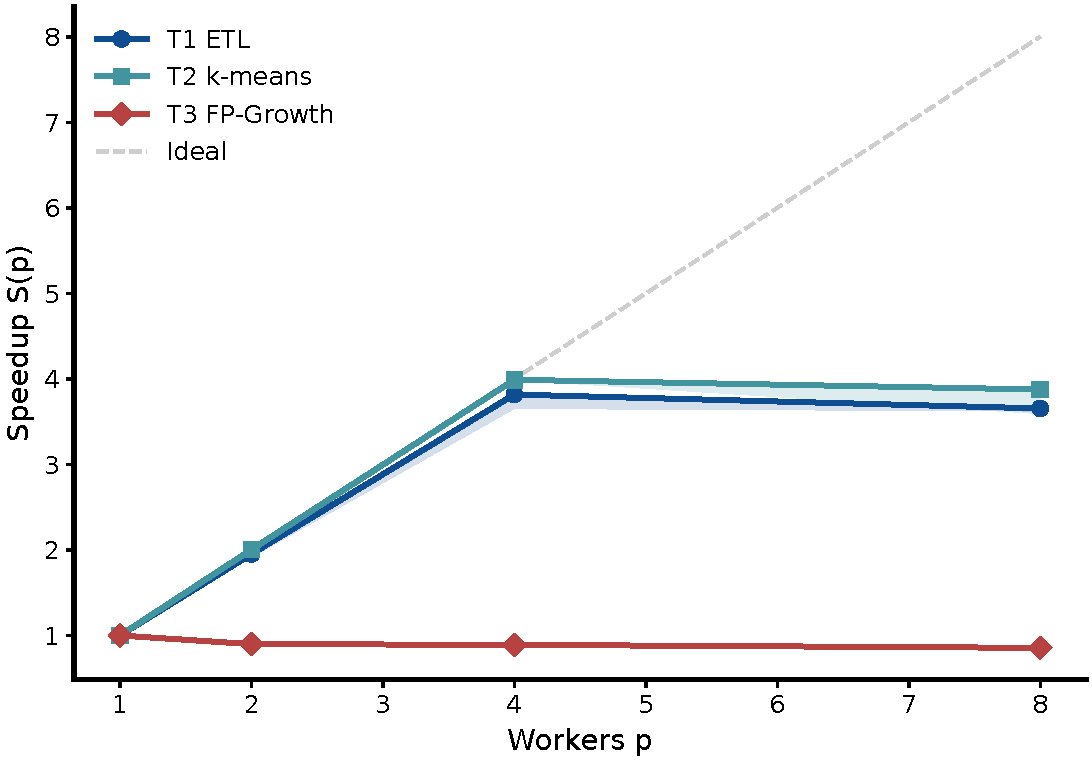
\includegraphics[width=0.86\textwidth]{fig09_speedup}
\caption{Warm-cache speedup. Bands convert the first and third quartiles of wall time with the same $T_1$. The dashed line is ideal speedup. $p = 8$ is eight workers on four cores.}
\label{fig:speedup}
\end{figure}

\begin{table}[ht]
\centering
\caption{ETL, twelve files of 2023, process pool, chunk size 1. Five repeats.}
\label{tab:t1}
\begin{tabular}{rrrr}
\toprule
$p$ & Median (s) & $S(p)$ & $E(p)$ \\
\midrule
1 & 52.135 & 1.00 & 1.000 \\
2 & 26.717 & 1.95 & 0.976 \\
4 & 13.658 & 3.82 & 0.954 \\
8 & 14.266 & 3.65 & 0.457 \\
\bottomrule
\end{tabular}
\end{table}

The process pool is close to linear through four workers: $S(2) = 1.95$ and $S(4) = 3.82$. Median system CPU moves from 25\% to 50\% to 100\%. At $p = 8$ the median rises from 13.658 s to 14.266 s and CPU stays at 100\%. There is no fifth core for the extra processes.

The same twelve files on a thread pool at $p = 4$ take 27.423 s, with median CPU 42.3\%. Relative to the one-process median of 52.135 s, that is $S = 1.90$. The process pool at the same $p$ takes 13.658 s and uses 100\% CPU. Pandas and Arrow release the GIL for part of the read and the numeric work, which is why four threads still beat one process. The cleaning rules keep the rest on one interpreter, which is why four processes beat four threads. The ETL uses processes for that reason.

A separate pure-Python loop, 400{,}000 tuples and no NumPy, checks the same mechanism on code that cannot release the GIL. Threads take 0.0179 s at $p = 1$ and 0.0195 s at $p = 4$. Processes take 0.292 s and 0.201 s. The pool costs more than the loop, so processes are slower in absolute time. The GIL evidence in Figure~\ref{fig:gil} is the flat thread bar. The pool decision uses the 27.423 s and 13.658 s above, not this figure.

\begin{figure}[ht]
\centering
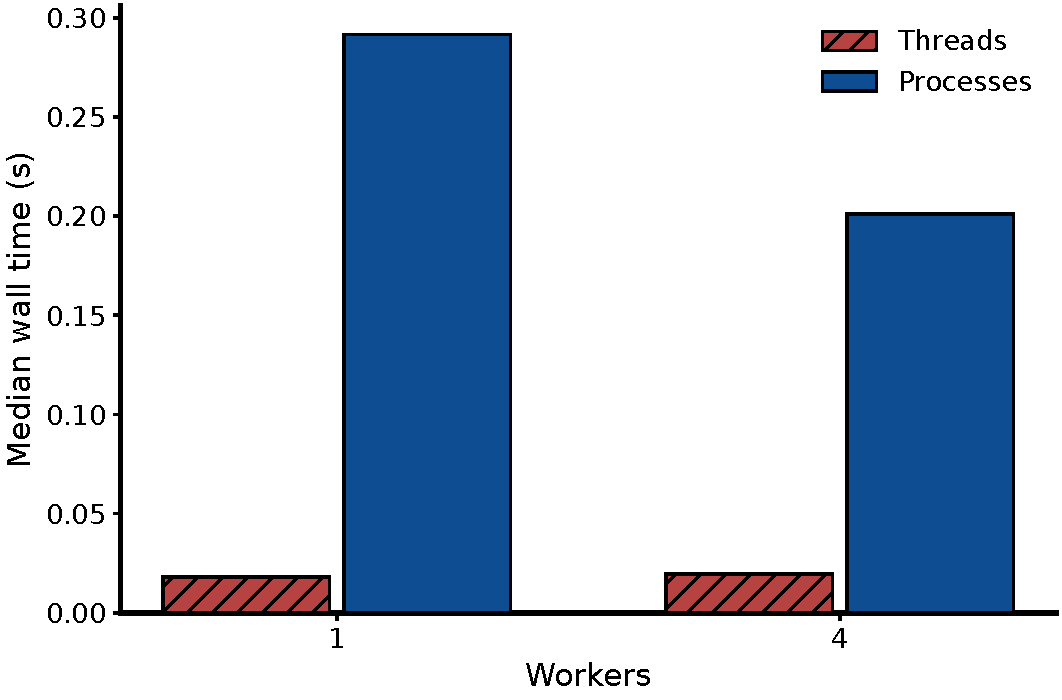
\includegraphics[width=0.72\textwidth]{fig12_gil}
\caption{Pure-Python row loop, 400{,}000 tuples. Threads stay near 0.02 s. Process startup dominates the same loop.}
\label{fig:gil}
\end{figure}

Chunk size is the number of files one worker receives in a batch. At $p = 4$, chunk size 1 takes 13.658 s. Chunk size 4 takes 17.038 s, and median CPU falls to 76.2\%. Chunk size 12 takes 49.668 s, and median CPU is 25.3\%. Twelve files in one chunk leave a single worker holding the year. The other three processes have nothing to run. A single file, January 2023, takes 4.579 s at $p = 1$ and 4.195 s at $p = 4$ ($S = 1.09$). One file cannot fill four workers, because the file is the unit of work.

\FloatBarrier
\subsection{Where the ETL time goes}
\label{sec:phases}

Figure~\ref{fig:phases} stacks three timers from the worker processes and draws wall time on top. The timers are summed across files and then divided by $p$. At $p = 1$ the medians are 1.600 s to read, 19.916 s to clean, and 26.527 s to aggregate. The stack is 48.0 s against a wall of 52.135 s. The gap is pool and interpreter time outside those three timers. Read is a small slice once the cache is warm.

\begin{figure}[ht]
\centering
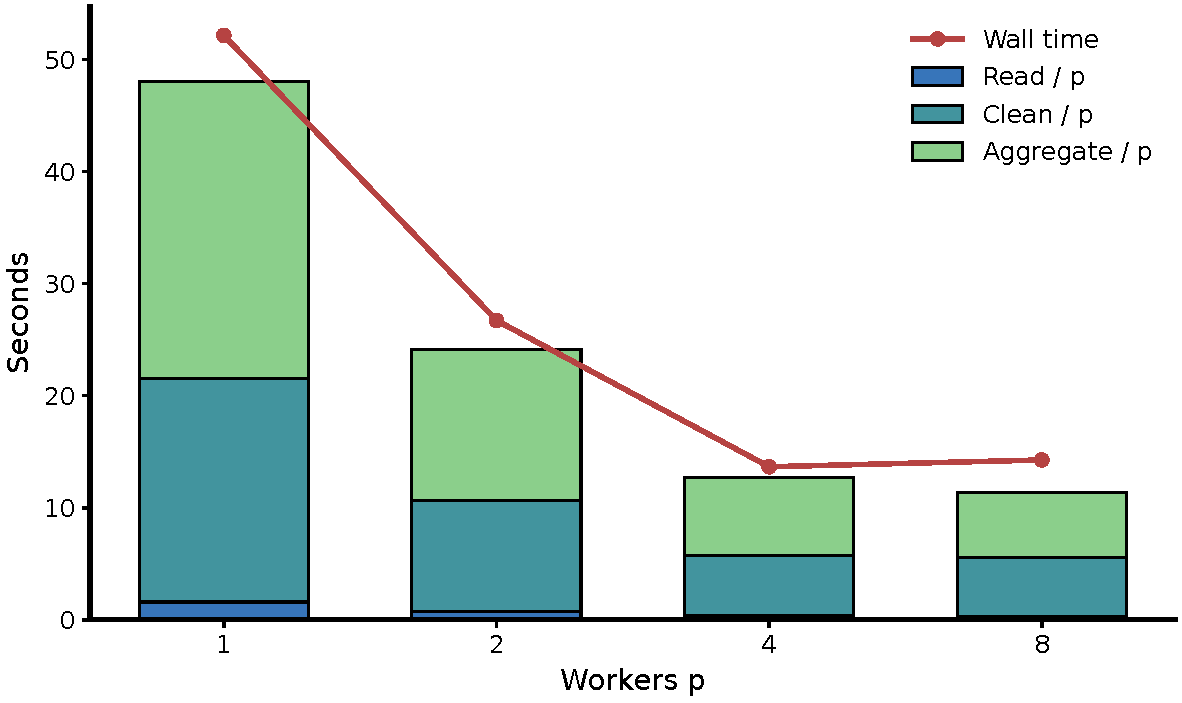
\includegraphics[width=0.86\textwidth]{fig10_phases}
\caption{ETL phases for the twelve files of 2023. Each bar is the summed phase CPU divided by $p$. The line is wall time. Through $p = 4$ the stack and the line fall together. At $p = 8$ the wall stops falling.}
\label{fig:phases}
\end{figure}

At $p = 4$ the summed clean and aggregate times stay near the serial sums (21.395 s and 27.954 s) while the wall falls to 13.658 s. At $p = 8$ those sums rise to 42.167 s and 46.218 s. Dividing by 8 makes the stack in the figure shorter than at $p = 4$, but the raw CPU grew, and the wall rose to 14.266 s. The extra processes wait on the same four cores. The bytes that cross the process boundary are the zone aggregates, not the trips. That reduce is small next to the clean and the aggregate, which is why $S(4)$ can reach 3.82. It does not remove the limit at four cores.

\FloatBarrier
\subsection{k-means speedup}
\label{sec:kmeans}

Table~\ref{tab:t2} is the timing kernel: 2{,}600{,}000 points, $k = 24$, 30 iterations, block 8{,}192, thread-local centroid update. This $k$ and these eight features are a compute load. They are not the $k = 4$ fit in Section~\ref{sec:clusters}.

\begin{table}[ht]
\centering
\caption{k-means, 2{,}600{,}000 points, $k = 24$, 30 iterations, block 8{,}192, thread-local update. Five repeats.}
\label{tab:t2}
\begin{tabular}{rrrr}
\toprule
$p$ & Median (s) & $S(p)$ & $E(p)$ \\
\midrule
1 & 6.428 & 1.00 & 1.000 \\
2 & 3.208 & 2.00 & 1.002 \\
4 & 1.611 & 3.99 & 0.997 \\
8 & 1.659 & 3.88 & 0.484 \\
\bottomrule
\end{tabular}
\end{table}

$S(2) = 2.00$ and $S(4) = 3.99$. The $p = 2$ point is slightly above 2. Replacing each median by the opposite quartile puts that speedup between 1.96 and 2.03, so the excess sits inside the repeat spread. At $p = 8$ the median rises from 1.611 s to 1.659 s. Eight threads are running on four pinned cores, and the wall stops falling.

Weak scaling keeps about 650{,}000 points per thread. The medians are 1.407 s at $p = 1$ (650{,}000 points), 1.575 s at $p = 2$ (1{,}300{,}000 points), and 1.624 s at $p = 4$ (2{,}600{,}000 points). Time rises 12\% and then 15\% while the row count quadruples. Ideal weak scaling would hold the time fixed. The 15\% rise is the departure from that line on this host.

Figure~\ref{fig:blocksize} varies the block at $p = 4$ on the same 2{,}600{,}000 points. Table~\ref{tab:block} lists the medians. The fastest block is 64 rows (1.594 s). The slowest is 262{,}144 rows (1.912 s). The range is 0.32 s. Between 1{,}024 and 65{,}536 rows the median stays inside 1.620--1.661 s, next to the 8{,}192-row point used in Table~\ref{tab:t2} (1.611 s). We do not read a preferred block size from that range. Worker count moves the median from 6.428 s to 1.611 s. Block size does not.

\begin{figure}[ht]
\centering
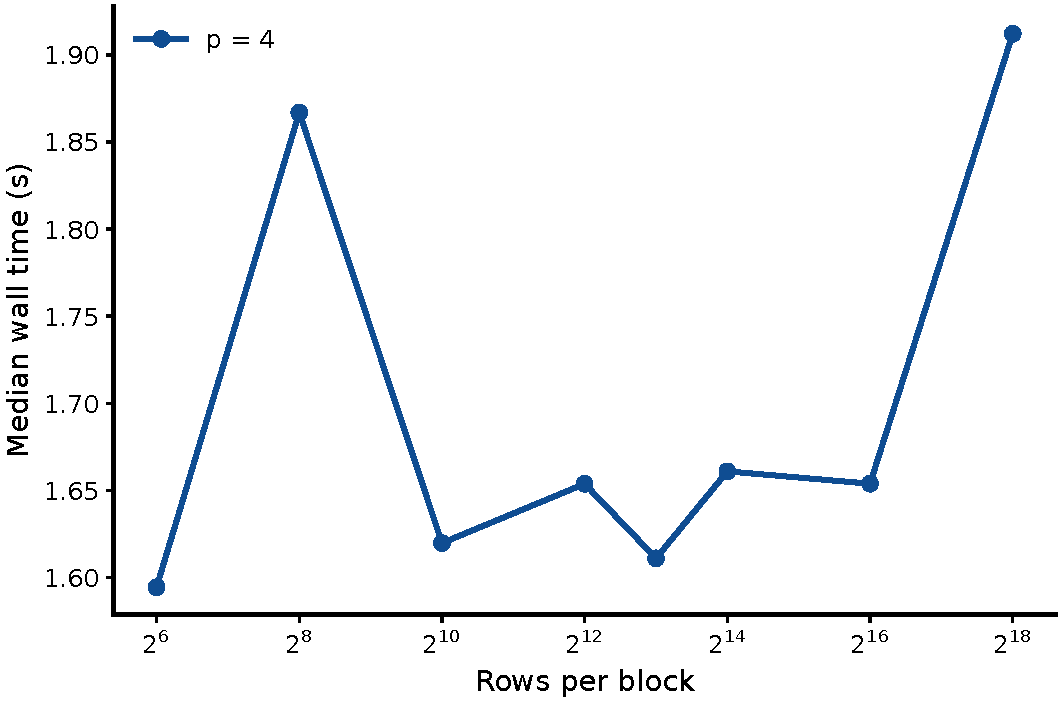
\includegraphics[width=0.78\textwidth]{fig11_blocksize}
\caption{k-means wall time against rows per block, $p = 4$, three repeats. The vertical range is 1.59--1.91 s.}
\label{fig:blocksize}
\end{figure}

\begin{table}[ht]
\centering
\caption{Block-size medians at $p = 4$. Three repeats, except 8{,}192 rows, which is the five-repeat entry from Table~\ref{tab:t2}.}
\label{tab:block}
\begin{tabular}{rr}
\toprule
Rows per block & Median (s) \\
\midrule
64 & 1.594 \\
256 & 1.867 \\
1,024 & 1.620 \\
4,096 & 1.654 \\
8,192 & 1.611 \\
16,384 & 1.661 \\
65,536 & 1.654 \\
262,144 & 1.912 \\
\bottomrule
\end{tabular}
\end{table}

\FloatBarrier
\subsection{A split that does not speed up}
\label{sec:fpgrowth}

FP-Growth was timed because the assignment lists association rules. We do not use the itemsets as a finding. On the inputs we tried, the frequent combinations restated long trips and payment type, and they did not add a travel pattern beyond Table~\ref{tab:clusters}. The timing result is still useful as a limit on this kind of parallelism.

The tree is built in the parent before the process pool starts. The pool then grows one conditional tree per frequent item~\cite{han2000}. Those tasks do not depend on each other. On 1{,}200{,}000 transactions at minimum support 0.02, the parent build dominates the measured time. Table~\ref{tab:t3} is the wall time. It rises from 1.497 s at one worker to 1.666 s, 1.681 s, and 1.750 s. $S(4) = 0.89$ and $S(8) = 0.86$. Median system CPU stays between 25.3\% and 25.6\% at every $p$. Extra processes do not occupy extra cores for most of that second and a half.

\begin{table}[ht]
\centering
\caption{FP-Growth, 1{,}200{,}000 transactions, minimum support 0.02. Five repeats.}
\label{tab:t3}
\begin{tabular}{rrrr}
\toprule
$p$ & Median (s) & $S(p)$ & $E(p)$ \\
\midrule
1 & 1.497 & 1.00 & 1.000 \\
2 & 1.666 & 0.90 & 0.449 \\
4 & 1.681 & 0.89 & 0.223 \\
8 & 1.750 & 0.86 & 0.107 \\
\bottomrule
\end{tabular}
\end{table}
